\documentclass[13pt, t]{beamer}
% Presento style file
\usepackage{config/presento}
\usepackage{hyperref}
%\graphicspath{ {images/} }

% custom command and packages
% custom packages
\usepackage{textpos}
\setlength{\TPHorizModule}{1cm}
\setlength{\TPVertModule}{1cm}

\newcommand\crule[1][black]{\textcolor{#1}{\rule{2cm}{2cm}}}



\usepackage{color, colortbl}

\title{\Large \hspace{-0.5cm} Жестовая лингвистика}
\author[shortname]{Аня Клезович, Гарик Мороз}
\institute[shortinst]{Лаборатория языковой конвергенции, НИУ ВШЭ, Москва}
\date{\begin{center} 24 июля 2019 \bigskip \\ {{\color{colorblue} \href{www.letnyayashkola.org/}{\large Летняя Школа}}\\ \vfill Презентация доступна здесь: {\large \href{https://tinyurl.com/yxbkl3ke}{tinyurl.com/yxbkl3ke}}} \end{center}}

\begin{document}

\begin{frame}[plain]
\maketitle
\end{frame}

\section{Введение} % Гарик

\begin{frame}{Мифы про ЖЯ:}
\pause
\begin{itemize}
    \item ЖЯ --- не один язык, а много языков 
\end{itemize}
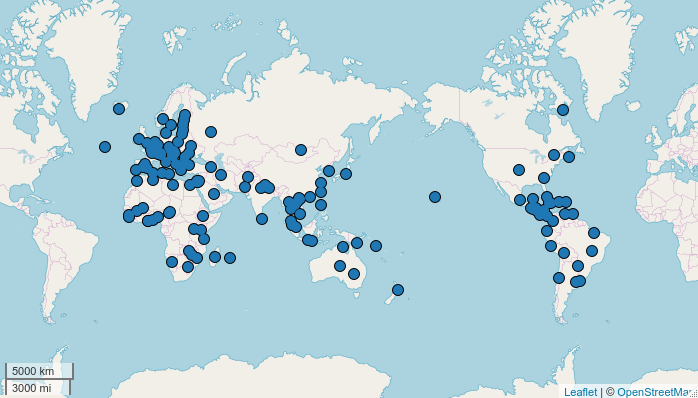
\includegraphics[width=\linewidth]{images/01-sign}
\end{frame}

\begin{frame}{Мифы про ЖЯ:}
\begin{itemize}
    \item ЖЯ --- не один язык, а много языков 
    \item Русский жестовый язык --- это не русский язык, передаваемый жестами 
\end{itemize}
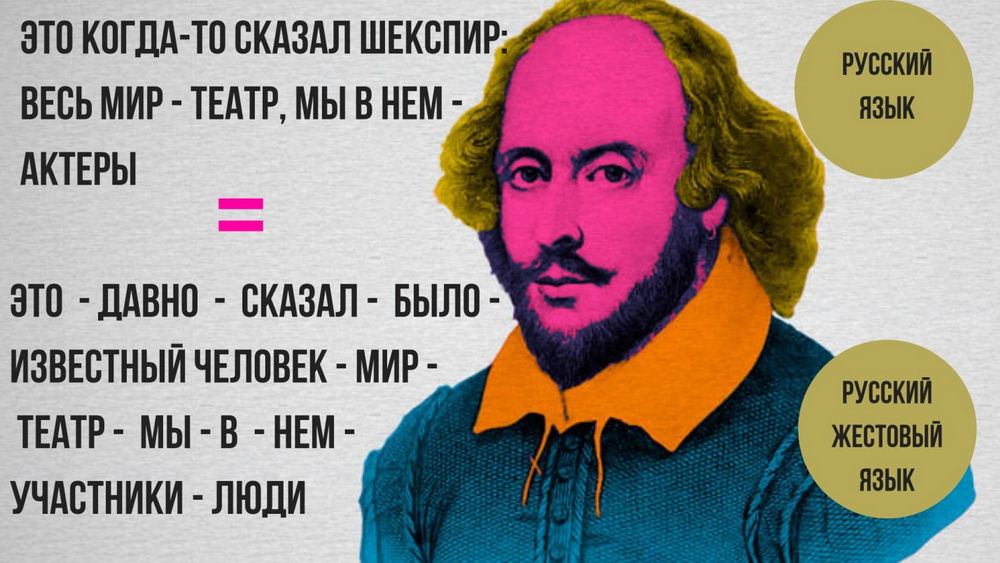
\includegraphics[width=\linewidth]{images/02-Rus-RSL}
\end{frame}


\begin{frame}{Мифы про ЖЯ:}
\begin{itemize}
    \item ЖЯ --- не один язык, а много языков 
    \item Русский жестовый язык --- это не русский язык, передаваемый жестами 
    \item Жестикуляция --- это не ЖЯ \pause
    \item В ЖЯ есть грамматика \pause
    \item Глухонемые? Нет, глухие \pause
    \item Существует жестовый театр, жестовые стихи и жестовое пение
\end{itemize}
\end{frame}

\section{История изучения} % Аня

\begin{frame}{Как все неправильно поняли Аристотеля}
    \begin{description}
        \item[16-ый век] может быть, все были не правы, но это не точно \pause
        \item[конец 18-ого --- начало 19-ого века] Возникновение школ для глухих (а именно 1760-е, Париж, Abbé Charles-Michel de l’Epée)
    \end{description}
    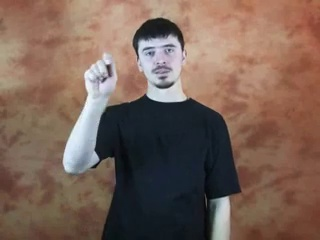
\includegraphics[width=0.49\linewidth]{images/delepe}
    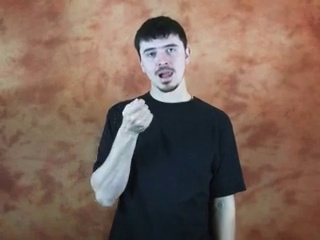
\includegraphics[width=0.49\linewidth]{images/delepe2}
\end{frame}

\begin{frame}{Как все неправильно поняли Аристотеля}
    \begin{description}
        \item[16-ый век] может быть, все были не правы, но это не точно
        \item[конец 18-ого --- начало 19-ого века] Возникновение школ для глухих (а именно 1760-е, Париж, Abbé Charles-Michel de l’Epée)
        \item[1864] Gallaudet University \pause
        \item[2/2 18-ого века] Орализм
        \item[1960 год] Стоуки написал первое лингвистическое исследование
    \end{description}
\end{frame}

\section{Грамматические особенности РЖЯ} % Гарик
\begin{frame}{Грамматика РЖЯ}
\begin{itemize}
    \item дактильная азбука
    \item нет падежей
    \item посессивная конструкция (мой мальчик)
    \item немануальное отрицание
    \item много повторов
    \item инициализированные жесты
    \item слабое различие между частями речи
    \item согласующиеся глаголы
    \item возможная нелинейность жестов
\end{itemize}
\end{frame}

\section{Иконичность и одновременность} % Аня
\begin{frame}{Чем жестовые языки принципиально отличаются от звучащих?}
\begin{itemize}
    \item Иконичность
    \item Одновременность
\end{itemize}
\end{frame}

\section{Фонетика и фонология} % Гарик

\begin{frame}{Звуковая сторона}
\begin{itemize}
    \item фонетические признаки:
    \begin{itemize}
        \item конфигурация
        \item место исполнения
        \item направление движения
        \item характер движения
        \item немануальный компонент
    \end{itemize}
    \item фонетические процессы (ассимиляции)
    \item можно выделять слоги
    \item можно выделять ударение
\end{itemize}
\end{frame}

\section{Автоматическое распознавание ЖЯ} % Аня
\begin{frame}{Автоматическое распознавание ЖЯ}
    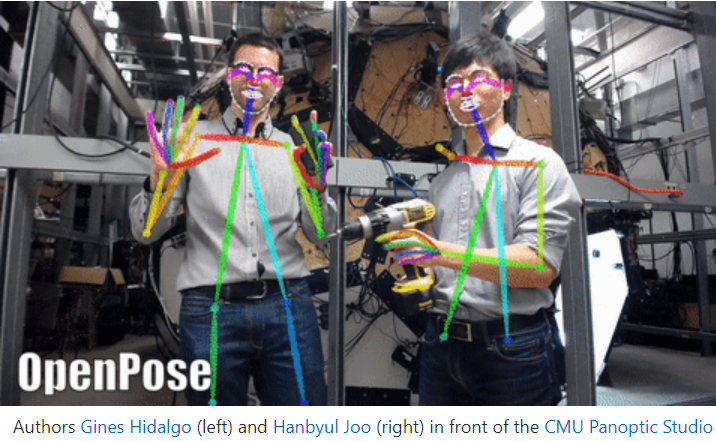
\includegraphics[width=\linewidth]{images/open-pose}
\end{frame}

\begin{frame}{Распознавание русского жестового языка}
    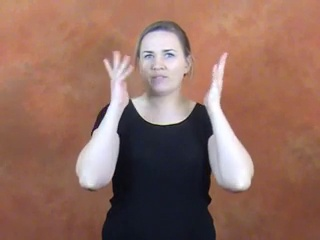
\includegraphics[width=0.49\linewidth]{images/vljubit'sja_frame1.jpg}
    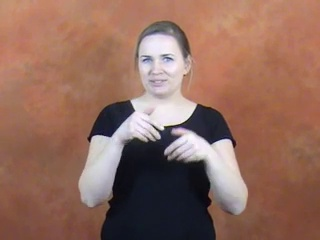
\includegraphics[width=0.49\linewidth]{images/vljubit'sja_frame2.jpg}
\end{frame}

\section{Песня, стихи и т. п.} % Гарик и Аня
\begin{frame}{Жестовая песня}
\begin{itemize}
    \item \href{https://www.youtube.com/watch?v=n-lNtm1lKsw}{Жестовая песня}
    \item \href{https://youtu.be/EuD2iNVMS_4?t=285}{Жестовая музыка}
\end{itemize}
\end{frame}

\begin{frame}{Где учить?}
Словарь на разных ЖЯ: spreadthesign.com
РЖЯ в Москве:
\begin{itemize}
    \item Центр образования глухих и жестового языка
    \item МГЛУ
    \item НИУ ВШЭ
\end{itemize}

\end{frame}

\framecard[colorblue]{{\color{colorwhite} \Large Пишите нам!\\
anna.klezovich@yandex.ru\\
agricolamz@gmail.com\\ 
\vfill Presentation is available here: \\tinyurl.com/yxbkl3ke}}

\end{document}